\documentclass[../fractal_dimensions_quasicrystals.tex]{subfiles}
\begin{document}


    	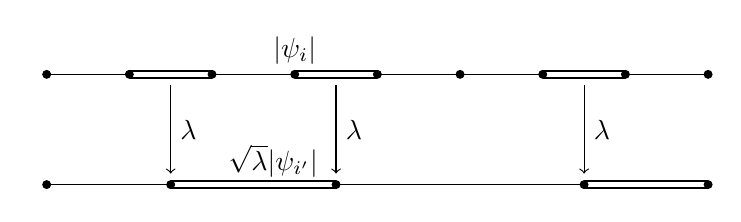
\begin{tikzpicture}[scale=.7]
    		\newcommand{\orig}{-1.5}
    		\newcommand{\trans}{1.5}
    		\newcommand{\vertspac}{-2.}
    		\newcommand{\vertsize}{0} % vertical span of the rectangles
    		\newcommand{\del}{.2}
    		\newcommand{\rad}{2pt} % radii of the circles

    		
    		% set the style of the strong bonds
    		\tikzset{
    			strong/.style={
    				double,
    				double distance=\rad,
    				line width=0.5pt
    				}
    		}
    	
    		% initial chain
    	
    		% bonds 
        	\draw[-] (\orig, 0)  node [left] {}  -- (\orig+\trans, 0);
			\draw[strong] (\orig+\trans,0) -- (\orig+2*\trans,0);
			\draw[-] (\orig+2*\trans,0) -- (\orig+3*\trans,0);	
			\draw[strong] (\orig+3*\trans,0) -- (\orig+4*\trans,0);
			\draw[-] (\orig+4*\trans,0) -- (\orig+5*\trans,0);
			\draw[-] (\orig+5*\trans,0) -- (\orig+6*\trans,0);
			\draw[strong] (\orig+6*\trans,0) -- (\orig+7*\trans,0);
			\draw[-] (\orig+7*\trans,0) -- (\orig+8*\trans,0);
    	
    		% sites
			\foreach \x in {0,...,8}
		      \filldraw (\orig+\x*\trans,0) circle (\rad); % node [below] {$\ket{\x}$};
		     
		     \filldraw (\orig+3*\trans,0) circle (0) node [above] {$|\psi_i|$};
		    
		    % arrows below rectangles
		    \draw [->] (\orig+1.5*\trans,-\vertsize-\del) -- (\orig+1.5*\trans,\vertspac+\del) node [midway, right] {$\lambda$};
		    \draw [->] (\orig+3.5*\trans,-\vertsize-\del) -- (\orig+3.5*\trans,\vertspac+\del) node [midway, right] {$\lambda$};
		    \draw [->] (\orig+6.5*\trans,-\vertsize-\del) -- (\orig+6.5*\trans,\vertspac+\del) node [midway, right] {$\lambda$};
		      
			% molecular chains
			
				\draw[-] (\orig, \vertspac) node [left] {} -- (\orig+1.5*\trans, \vertspac);
				\draw[strong] (\orig+1.5*\trans,\vertspac) -- (\orig+3.5*\trans, \vertspac);
				\draw[-] (\orig+3.5*\trans, \vertspac) -- (\orig+6.5*\trans, \vertspac);
				\draw[strong] (\orig+6.5*\trans, \vertspac) -- (\orig+8*\trans, \vertspac);
				
				\filldraw (\orig,\vertspac) circle (\rad);
				\filldraw (\orig+1.5*\trans,\vertspac) circle (\rad);
				\filldraw (\orig+3.5*\trans,\vertspac) circle (\rad) node [shift={(-0.8,0.3)}] {$\sqrt{\lambda} |\psi_{i'}|$};
				\filldraw (\orig+6.5*\trans,\vertspac) circle (\rad);
				\filldraw (\orig+8*\trans,\vertspac) circle (\rad);
			
		\end{tikzpicture}

\end{document}